\chapter{Related Work}
\label{ch:related-work}

\section{YOLO11}
\label{related_work_yolo11}

Object detection is a fundamental task in computer vision that aims to localize and classify objects within images. Among the numerous object detection frameworks proposed in recent years, \acrfull{yolo} was a major breakthrough. By formulating object detection as a single-stage prediction problem, \acrshort{yolo} enables efficient deployment in time-critical applications such as autonomous vehicles, robotics, surveillance, and intelligent transportation systems. Over the years, the \acrshort{yolo} family has undergone continuous development, with each generation addressing limitations of previous versions. Table~\ref{tab:yolo_evolution} summarizes the evolution of \acrshort{yolo} models and their key contributions. \cite{yolov11}

Building upon these developments, \acrshort{yolo}11 introduces the following further improvements in both efficiency and detection accuracy while preserving the real-time characteristics that have made the \acrshort{yolo} family successful \cite{yolo11_ultralytics}:
\begin{itemize}
\item \textbf{Enhanced feature extraction:} \acrshort{yolo}11 employs an improved backbone and neck architecture, resulting in stronger feature extraction capabilities for more precise object detection and improved performance on complex computer vision tasks.
\item \textbf{Optimized efficiency and speed:} The model introduces refined architectural designs and optimized training pipelines that increase processing speed while maintaining a favorable balance between detection accuracy and computational efficiency.
\item \textbf{Greater accuracy with fewer parameters:} According to the Ultralytics documentation, \acrshort{yolo}11 medium achieves a higher \acrshort{map} on the COCO dataset while using 22\% fewer parameters than \acrshort{yolo}v8 medium, improving computational efficiency without sacrificing accuracy.
\item \textbf{Adaptability across environments:} \acrshort{yolo}11 can be deployed across a wide range of environments, including edge devices, cloud platforms, and systems equipped with NVIDIA GPUs, enabling flexible deployment scenarios.
\item \textbf{Broad task support:} Beyond object detection, \acrshort{yolo}11 supports instance segmentation, image classification, pose estimation, and oriented bounding box (OBB) detection within a unified framework.
\end{itemize}

\begin{table}[htbp]
    \centering
    \begin{tabular}{p{1.6cm}p{0.9cm}p{4.2cm}p{4.5cm}p{1.6cm}}
\hline \textbf{Release} & \textbf{Year} & \textbf{Tasks} & \textbf{Key Contributions} \\ \hline YOLO & 2015 & Object Detection, Basic Classification & Single-stage object detector \\ YOLOv2 & 2016 & Object Detection, Improved Classification & Multi-scale training, dimension clustering \\ YOLOv3 & 2018 & Object Detection, Multi-scale Detection & SPP block, Darknet-53 backbone \\ YOLOv4 & 2020 & Object Detection, Basic Object Tracking & Mish activation, CSPDarknet-53 backbone \\ YOLOv5 & 2020 & Object Detection, Basic Instance Segmentation & Anchor-free detection, SWISH activation, PANet \\ YOLOv6 & 2022 & Object Detection, Instance Segmentation & Self-attention, anchor-free object detection \\ YOLOv7 & 2022 & Object Detection, Object Tracking, Instance Segmentation & Transformers, E-ELAN reparameterization \\ YOLOv8 & 2023 & Object Detection, Instance Segmentation, Panoptic Segmentation, Keypoint Estimation & GANs, anchor-free detection \\ YOLOv9 & 2024 & Object Detection, Instance Segmentation & PGI and GELAN \\ YOLOv10 & 2024 & Object Detection & Consistent dual assignments for NMS-free training
\\ \hline 
    \end{tabular}
    \caption{Evolution of YOLO models up to YOLOv10. Adapted from Table 1 in \cite{yolov11}.}
    \label{tab:yolo_evolution} \footnotesize
\end{table}



\section{EdgeCrafter}
\label{related_work_edgecrafter}

According to Liu et al. \cite{edgecrafter}, while \acrfull{cnn} based architectures such as \acrshort{yolo} continue to dominate resource-constrained dense prediction tasks on edge devices, compact \acrfull{vit} often struggle to achieve comparable accuracy-efficiency trade-offs. The authors explain that this performance gap is not necessarily caused by an inherent incompatibility between \acrshort{vit}s and dense prediction tasks, but rather by insufficient task-specific representation learning in small-scale transformer models. To address this limitation, the authors propose \emph{EdgeCrafter}, a unified compact \acrshort{vit} framework for edge dense prediction that consists of: 
\begin{itemize}
\item \textbf{ECDet} for object detection,
\item \textbf{ECInsSeg} for instance segmentation,
\item \textbf{ECPose} for human pose estimation.
\end{itemize}

The EdgeCrafter framework is centered around the object detection model \emph{ECDet}. Its primary objective is to combine the representational capabilities of transformer-based architectures with the computational efficiency required for deployment on edge devices. In contrast to larger transformer-based detectors that often rely on extensive pretraining and large model capacities, EdgeCrafter focuses on compact architectures optimized for strict parameter and computational budgets. \cite{edgecrafter}

\subsection{Task-Specialized Knowledge Distillation}
A central contribution of EdgeCrafter is its task-specialized distillation strategy. The complete training pipeline is shown in Figure~\ref{fig:edgecrafter_training}.

\begin{figure}[htbp]
\centering
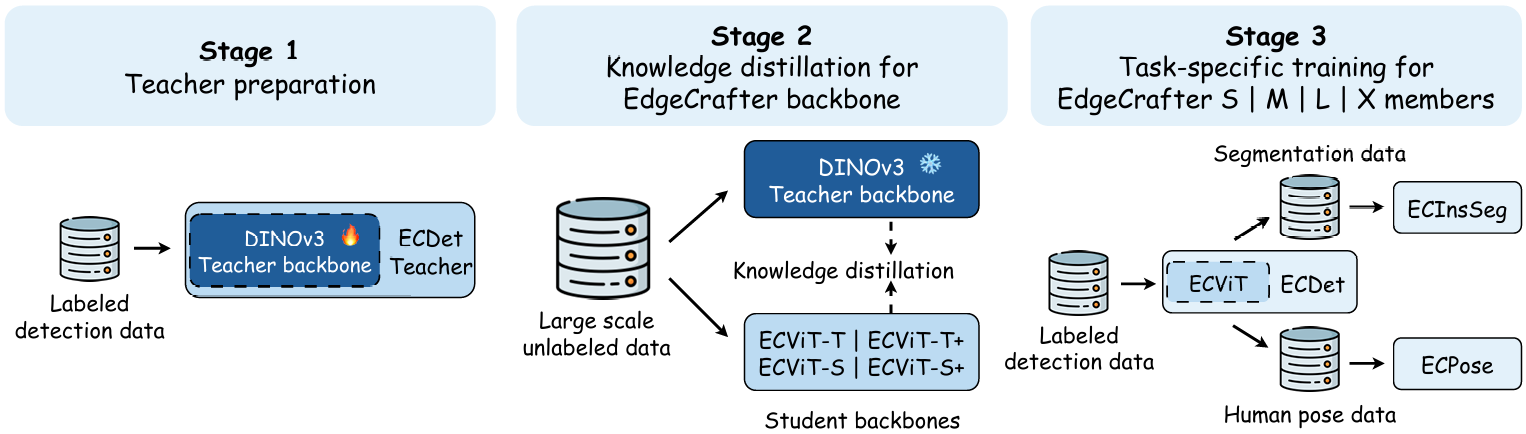
\includegraphics[width=\textwidth]{content/figures/edgecrafter_training.png}
\caption{Three-stage EdgeCrafter training pipeline. \cite{edgecrafter}}
\label{fig:edgecrafter_training}
\end{figure}

The training procedure consists of three stages \cite{edgecrafter}:

\begin{enumerate} \item \textbf{Teacher preparation:} A large DINOv3-pretrained Vision Transformer is first adapted to object detection, creating a task-specialized teacher model referred to as ECDet Teacher.

\item \textbf{Knowledge distillation:} The teacher's feature representations are distilled to compact \emph{ECViT} student backbones through feature alignment on a large image collection.

\item \textbf{Task-specific training:} The distilled student backbone is subsequently used to train \emph{ECDet}, \emph{ECInsSeg}, and \emph{ECPose} for their respective downstream tasks.

\end{enumerate}

The authors emphasize that object detection serves as the primary representation-learning task. The learned detection-oriented representations are then transferred directly to instance segmentation and human pose estimation through task-specific prediction modules \cite{edgecrafter}. Experimental results reported in the paper indicate that this task-specialized distillation strategy substantially improves downstream performance compared to conventional generic pretraining approaches.

\subsection{Architecture}

Figure~\ref{fig:edgecrafter_architecture} illustrates the overall ECDet architecture. The model consists of three main components: a compact transformer backbone ECViT, followed by an encoder and a decoder for set-based object prediction \cite{edgecrafter}.

\begin{figure}[htbp]
\centering
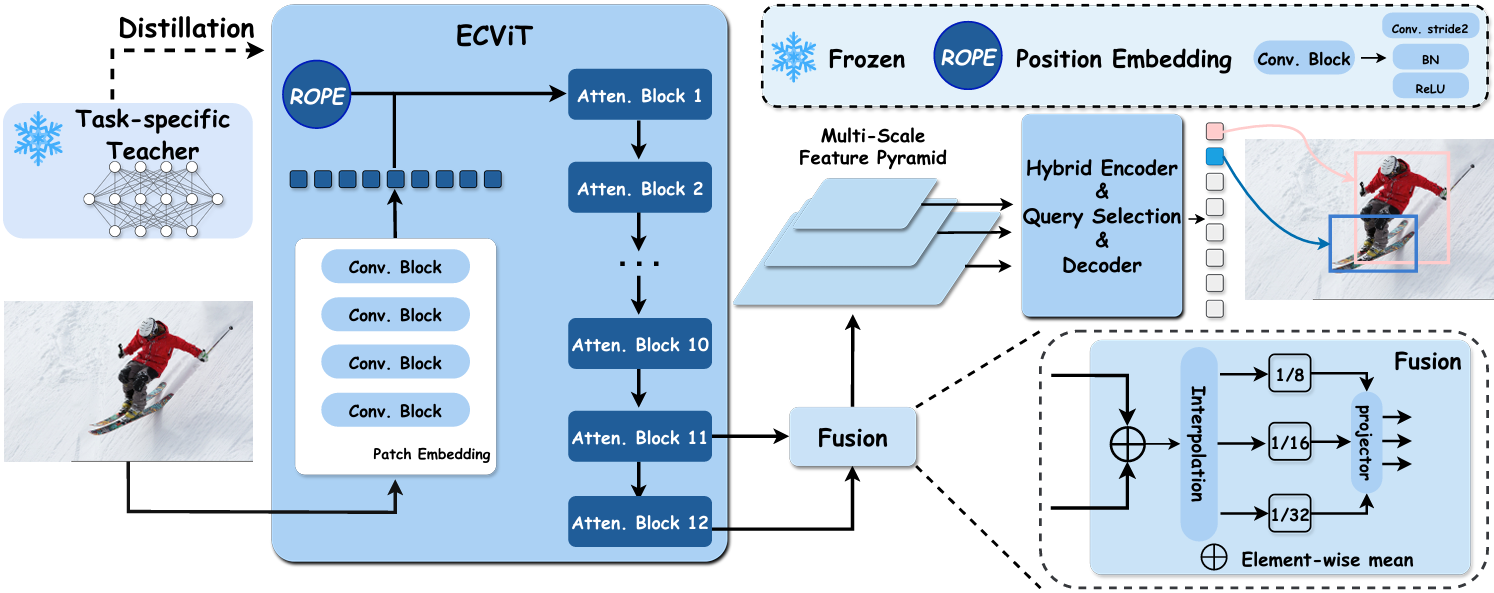
\includegraphics[width=\textwidth]{content/figures/edgecrafter_architecture.png}
\caption{Overview of the ECDet architecture. \cite{edgecrafter}}
\label{fig:edgecrafter_architecture}
\end{figure}

A key modification compared to conventional Vision Transformers is the replacement of the standard patch embedding layer with a lightweight convolutional stem consisting of four convolutional layers. According to the authors, this design preserves local image structures more effectively and improves dense localization performance. The generated feature representation is subsequently processed by a sequence of transformer attention blocks forming the EC\acrshort{vit} backbone. \cite{edgecrafter}

Since Vision Transformers do not naturally provide hierarchical feature pyramids, EdgeCrafter explicitly constructs a multi-scale feature representation from the final transformer layers. Rather than employing computationally expensive feature pyramid networks, the model generates feature maps at multiple resolutions using interpolation and lightweight convolutional projection layers. The resulting multi-scale feature representations are subsequently processed by an object detection head consisting of an encoder and a decoder. Following the design choices of RT-DETR, EdgeCrafter adopts a multi-scale hybrid encoder for feature aggregation and query selection. The decoder follows the DETR paradigm and predicts object classes and bounding boxes directly from the selected object queries. All three variants share the same distilled backbone representation and differ only in their lightweight task-specific prediction heads \cite{edgecrafter}.

\subsection{Performance Compared to State-of-the-Art Methods}

A major contribution of EdgeCrafter is its strong accuracy-efficiency trade-off. Figure~\ref{fig:edgecrafter_performance} compares the object detection performance of ECDet with several state-of-the-art detectors, including RT-DETRv4, RF-DETR, and YOLO26 \cite{edgecrafter}.

\begin{figure}[htbp]
\centering
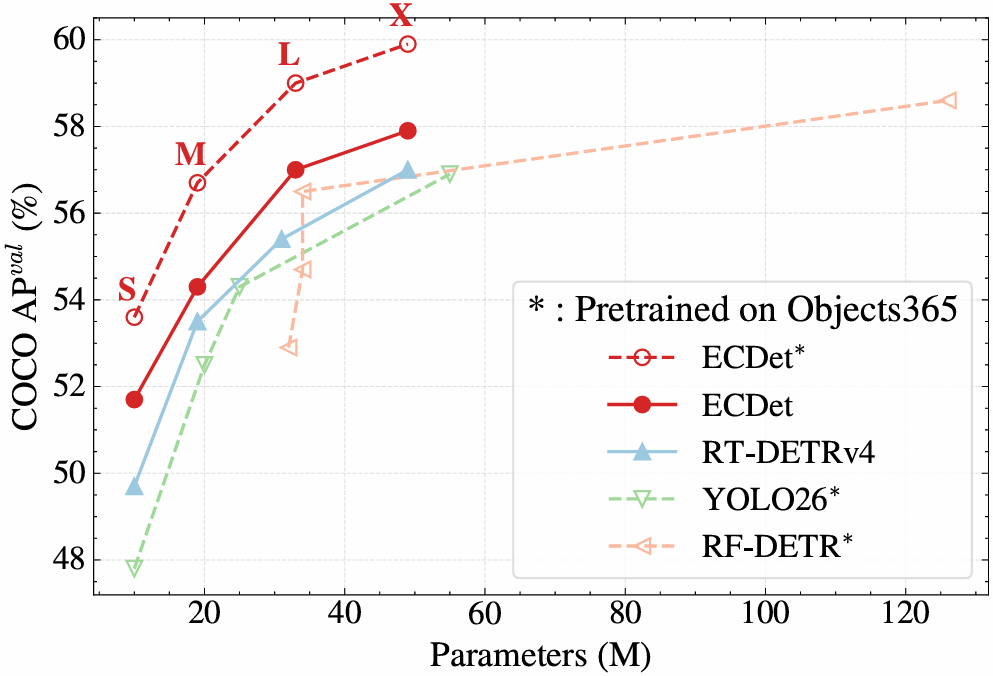
\includegraphics[width=0.75\textwidth]{content/figures/edgecrafter_result.png}
\caption{Comparison of COCO object detection performance and model size. Methods marked with * are pretrained on Objects365. \cite{edgecrafter}} \label{fig:edgecrafter_performance}
\end{figure}

The results demonstrate that ECDet achieves a favorable balance between model size and detection accuracy. For example, the smallest ECDet variant achieves 51.7 AP on the COCO validation dataset while using 10 million parameters. With additional Objects365 pretraining, ECDet-S reaches 53.6 AP. Compared to YOLO26-S, ECDet-S achieves higher detection performance at a comparable parameter count. The EdgeCrafter benchmark additionally reports competitive or superior performance compared to RT-DETRv4 and several other recent transformer-based detectors across multiple model scales. Similar observations are reported for the instance segmentation and human pose estimation variants ECInsSeg and ECPose, indicating that the distilled backbone transfers effectively across multiple dense prediction tasks. \cite{edgecrafter}

Overall, the results presented by Liu et al. suggest that compact Vision Transformers can achieve state-of-the-art performance in edge dense prediction when combined with task-specialized distillation and an architecture specifically designed for efficiency-constrained deployment scenarios \cite{edgecrafter}.